\documentclass[12pt]{beamer}
\usepackage[utf8]{inputenc}
\usepackage[frenchb]{babel}
\usepackage{listings}
\usepackage{tabu}
\usepackage{booktabs}
\beamertemplatenavigationsymbolsempty
\AtBeginSection[]
{
    \begin{frame}
    \frametitle{Table des matières}
    \tableofcontents[currentsection]
    \end{frame}
}
\lstset{language=C++, basicstyle=\footnotesize, frame=single}
\newcommand{\gray}{\textcolor{gray}}
\newcommand{\On}{\gray{O(n)}}

\title{Structures de données linéaires}
\subtitle{Tableaux, vecteurs, listes chaînées}
\author{Training beOI}
\institute{
\includegraphics[height=12em]{../shared-img/beoi-logo}}

\begin{document}

\frame{\titlepage}



\section{Tableaux et variantes}

\begin{frame}[fragile]
\frametitle{Tableau}
\begin{lstlisting}
#define MAXN 10000
int tab[MAXN];

int main()
{
    tab[1234] = 100;
    tab[1234]; // 100
    tab[5678]; // 0
}
\end{lstlisting}
\begin{itemize}
\item Taille fixée à la compilation
\item Accès à un élément arbitraire: $O(1)$
\item Truc: en-dehors d'une fonction, initialisé à zéro
\end{itemize}
\end{frame}

\begin{frame}[fragile]
\frametitle{Bitset}
\begin{lstlisting}
bitset<MAXN> tab; // bool tab[MAXN];
tab[1234] = true;

bitset<4> b1(string("1100")),
          b2(string("0101"));
b1 | b2; // 1101
b1 & b2; // 0100
b1 >> 1; // 0110
\end{lstlisting}
\begin{itemize}
\item Comme un tableau de booléens
\item 8x plus compact
\item Opérations bit-à-bit 64x plus rapides
\item Voir manuel pour la liste des opérations
\end{itemize}
\end{frame}

\begin{frame}[fragile]
\frametitle{Tableau dynamique: fonctionnement}
{\setlength{\parskip}{.9em}
Si plus de place, multiplier par 2

\def\arraystretch{1.3}

\begin{tabu} to .175\textwidth {|X[c]|X[c]|}
\hline
1 & \\
\hline
\end{tabu}
\hfill Capacité = 2

\begin{tabu} to .175\textwidth {|X[c]|X[c]|}
\hline
1 & 2 \\
\hline
\end{tabu}

\begin{tabu} to .35\textwidth {|X[c]|X[c]|X[c]|X[c]|}
\hline
1 & 2 & 3 & \\
\hline
\end{tabu}
\hfill Capacité = 4

\begin{tabu} to .35\textwidth {|X[c]|X[c]|X[c]|X[c]|}
\hline
1 & 2 & 3 & 4 \\
\hline
\end{tabu}

\begin{tabu} to .7\textwidth {|X[c]|X[c]|X[c]|X[c]|X[c]|X[c]|X[c]|X[c]|}
\hline
1 & 2 & 3 & 4 & 5 & & & \\
\hline
\end{tabu}
\hfill Capacité = 8} %\setlength
\end{frame}

\begin{frame}[fragile]
\frametitle{Tableau dynamique: en pratique}
\begin{lstlisting}
vector<int> vec(8, -1); // initialize to -1
vec[5] += vec[2];       // -2
vec.push_back(5);
vec.push_back(19);
vec.pop_back();
vec.back();             // 5
\end{lstlisting}
\begin{itemize}
\item Taille augmente et diminue
\item Accès à un élément arbitraire: $O(1)$
\item Ajout/suppression d'un élément \textbf{à la fin}: $O(1)$
\item Ajout/suppression autre part: $O(n)$
\end{itemize}
\end{frame}

\section{Listes chaînées}

\begin{frame}[fragile]
\frametitle{Liste chaînée: concept}
Des nœuds reliés par des liens (pointeurs)
\begin{figure}
\centering
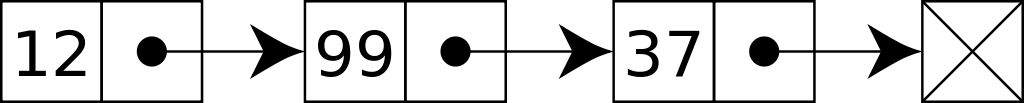
\includegraphics[width=.8\textwidth]{img/singly-linked}
\end{figure}
\begin{itemize}
\item Chaque nœud sait où est le prochain
\item Les nœuds ne sont plus côte à côte
\end{itemize}
\begin{lstlisting}
struct Node
{
    int value;
    Node *next; // link (pointer)
};
\end{lstlisting}
\end{frame}

\begin{frame}[fragile]
\frametitle{Liste chaînée: parcours}
Commencer au premier nœud et suivre les liens
\begin{figure}
\centering
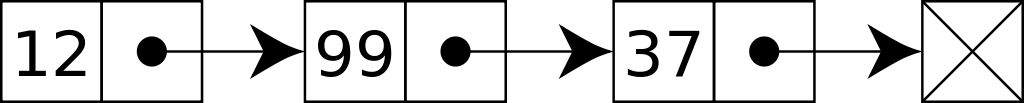
\includegraphics[width=.6\textwidth]{img/singly-linked}
\end{figure}
Dans le dernier nœud le lien vaut NULL:
\begin{lstlisting}
Node *cur = start;   // always keep the first node!
while (cur != NULL)
{
    cur->value;      // access value
    cur = cur->next; // switch pointer to next
}
\end{lstlisting}
\end{frame}

\begin{frame}[fragile]
\frametitle{Liste chaînée: ajout}
Seulement deux liens à changer
\begin{figure}
\centering
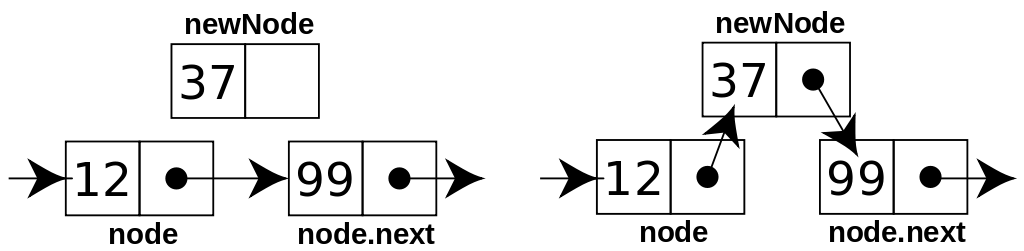
\includegraphics[width=.9\textwidth]{img/insert-node}
\end{figure}
\begin{lstlisting}
void insertAfter(Node *node, Node *new_node)
{
    new_node->next = node->next;
    node->next = new_node;
}
\end{lstlisting}
\end{frame}

\begin{frame}[fragile]
\frametitle{Liste chaînée: suppression}
Changer le lien et supprimer
\begin{figure}
\centering
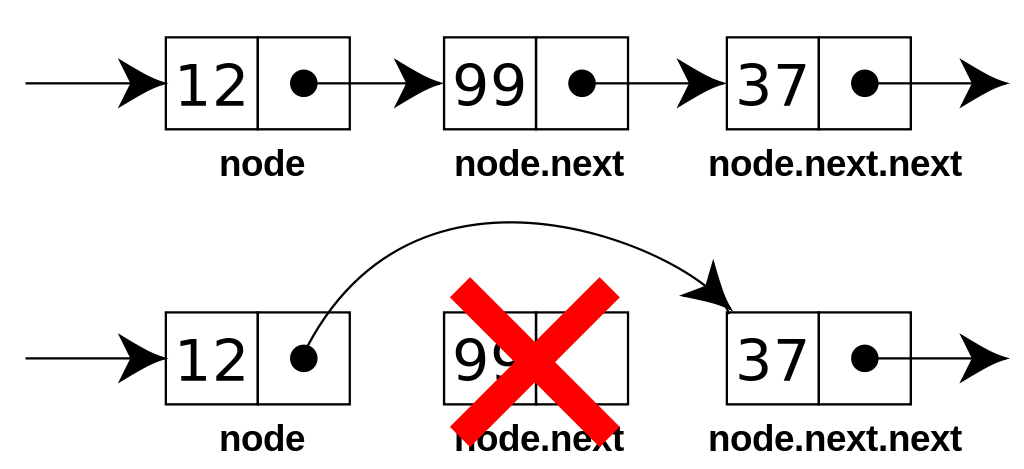
\includegraphics[width=.6\textwidth]{img/remove-node}
\end{figure}
\begin{lstlisting}
void removeAfter(Node *node)
{
    Node *toRemove = node->next;
    node->next = node->next-next; // bypass
    free(toRemove);
}
\end{lstlisting}
\end{frame}

\begin{frame}[fragile]
\frametitle{Liste chaînée: limitations}
\begin{figure}
\centering
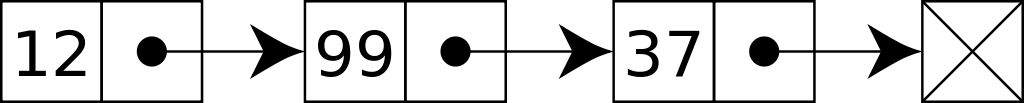
\includegraphics[width=.8\textwidth]{img/singly-linked}
\end{figure}
Avec une liste (simplement) chaînée:
\begin{itemize}
\item Ajout/suppression au début: $O(1)$
\item Ajout/suppression à une position \textbf{donnée}: $O(1)$
\end{itemize}
Si on retient la fin aussi:
\begin{itemize}
\item Ajout à la fin: $O(1)$
\item Suppression à la fin: pas possible, $O(n)$
\end{itemize}
\end{frame}

\begin{frame}[fragile]
\frametitle{Liste doublement chaînée}
Des liens dans les deux sens!
\begin{figure}
\centering
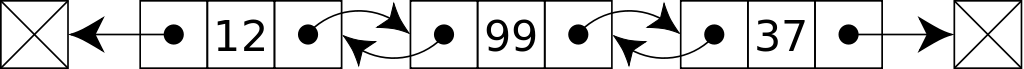
\includegraphics[width=.8\textwidth]{img/doubly-linked}
\end{figure}
\begin{itemize}
\item Parcours dans les deux sens
\item Suppression à la fin en $O(1)$
\item Un peu plus lourd
\end{itemize}
\begin{lstlisting}
struct Node
{
    int value;
    Node *prev, *next; // two pointers
};
\end{lstlisting}
\end{frame}

\begin{frame}[fragile]
\frametitle{Listes chaînée: en pratique}
\begin{lstlisting}
list<int> l;
list<int>::iterator it;

l.push_back(3);  // 3
it = l.begin();  // ^ points to 3
l.push_back(4);  // 3 4
l.push_front(1); // 1 3 4
l.insert(it, 2); // 1 2 3 4 (inserts before 3)
l.pop_front();   // 2 3 4
l.pop_back();    // 2 3
\end{lstlisting}
\begin{itemize}
\item Les \texttt{list<>} sont doublement chaînées
\item Retenir les positions avec des \texttt{iterator}
\item Tout en $O(1)$
\end{itemize}
\end{frame}

\section{File et pile}

\begin{frame}
\frametitle{File: concept}
\begin{itemize}
\item Faire la file dans un magasin
\item On ajoute à la fin, on enlève au début
\item Premier arrivé premier servi (First In First Out)
\end{itemize}
\begin{figure}
\centering
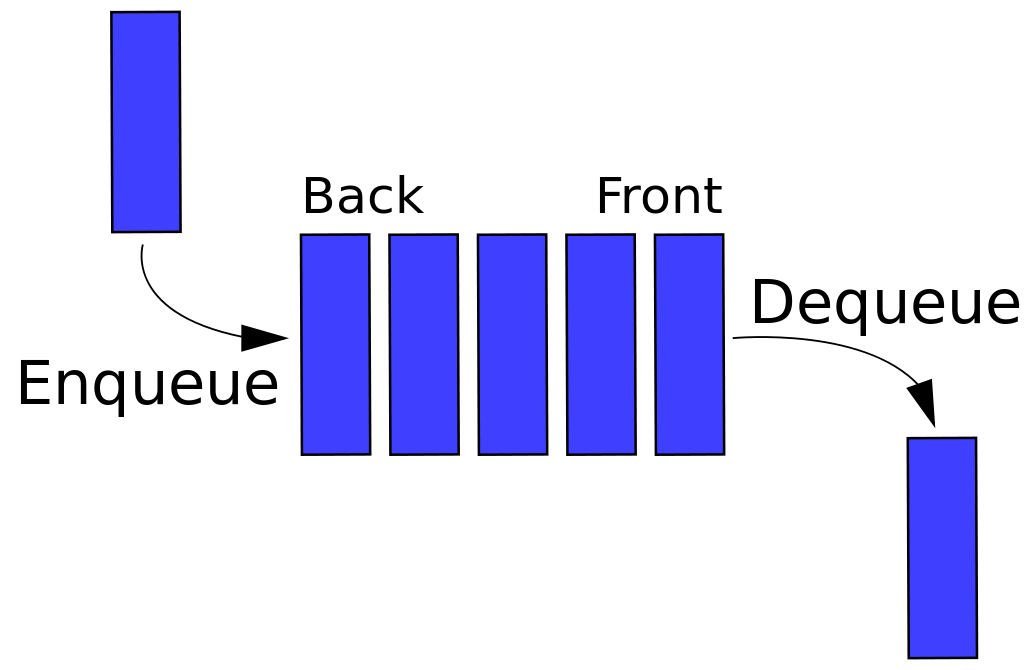
\includegraphics[width=.6\textwidth]{img/queue}
\end{figure}
\end{frame}

\begin{frame}[fragile]
\frametitle{File: en pratique}
\begin{itemize}
\item Ajouter à la fin, enlever au début $\Rightarrow$ liste chaînée
\item Tout en $O(1)$
\item On utilise \texttt{queue<>} (fait pour ça)
\end{itemize}
\begin{lstlisting}
queue<int> q;
q.push(1);
q.push(2);
q.front(); // 1
q.pop();
q.front(); // 2
\end{lstlisting}
\end{frame}

\begin{frame}
\frametitle{Pile: concept}
\begin{itemize}
\item Pile de crêpes
\item On ajoute au-dessus, on enlève au-dessus
\item Dernière cuite première mangée (Last In First Out)
\end{itemize}
\begin{figure}
\centering
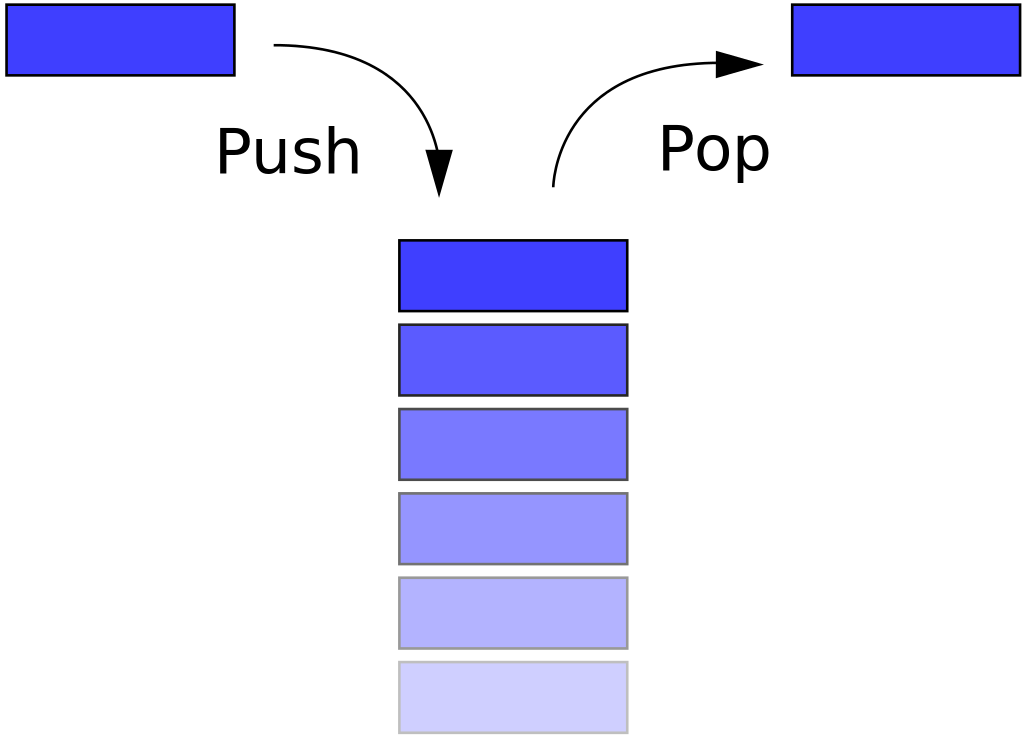
\includegraphics[width=.5\textwidth]{img/stack}
\end{figure}
\end{frame}

\begin{frame}[fragile]
\frametitle{Pile: en pratique}
\begin{itemize}
\item Ajouter et enlever à la fin $\Rightarrow$ liste chaînée \emph{ou vecteur}
\item Tout en $O(1)$
\item On utilise \texttt{stack<>} (fait pour ça)
\end{itemize}
\begin{lstlisting}
stack<int> q;
q.push(1);
q.push(2);
q.top(); // 2
q.pop();
q.top(); // 1
\end{lstlisting}
\end{frame}

\section{Choisir la bonne structure}

\begin{frame}
\frametitle{Choix: structures spéciales}
Structures pour besoins spéciaux:
\begin{itemize}
\item Ajoute d'un côté et on enlève de l'autre $\Rightarrow$ \textbf{file}
\item Enlève et ajoute d'un même côté $\Rightarrow$ \textbf{pile}
\item Booléens, opérations spéciales (et, ou, shift, ...) $\Rightarrow$ \textbf{bitset}
\end{itemize}

~

Sinon, voir slide suivante!
\end{frame}

\begin{frame}
\frametitle{Choix: tableaux, vecteurs, listes chaînées}
``Ajout'' = ajout ou suppression
\begin{center}
\begin{tabu}{l|cccc}
\toprule
Structure & Indexation & Ajout fin & Ajout milieu \\
\midrule
Tableau & $O(1)$ & $\On$ & $\On$ \\
Vecteur & $O(1)$ & $O(1)$ & $\On$ \\
Liste chaînée & $\On$ & $O(1)$ & $O(1)$ \\
\bottomrule
\end{tabu}
\end{center}
\begin{itemize}
\item Ajout au milieu nécessaire (rare) $\Rightarrow$ \textbf{liste chaînée}
\item Taille maximale inconnue $\Rightarrow$ \textbf{vecteur}
\item Tous les autres cas $\Rightarrow$ \textbf{tableau} (plus rapide)
\end{itemize}
\end{frame}

\begin{frame}
\frametitle{Source des figures}
\begin{itemize}
\item \url{https://commons.wikimedia.org/wiki/File:Singly-linked-list.svg}
\item \url{https://commons.wikimedia.org/wiki/File:CPT-LinkedLists-addingnode.svg}
\item \url{https://en.wikipedia.org/wiki/File:CPT-LinkedLists-deletingnode.svg}
\item \url{https://en.wikipedia.org/wiki/File:Doubly-linked-list.svg}
\item \url{https://en.wikipedia.org/wiki/File:Data_Queue.svg}
\item \url{https://en.wikipedia.org/wiki/File:Data_stack.svg}
\end{itemize}
\end{frame}

\end{document}
